\subsection{BERT} \label{sec:bert}

Bidirectional Encoder Representations from Transformers (BERT) is a pre-trained
encoder-only Transformer model introduced in \cite{devlin2019bert}, which aims
to generate contextual representations of textual input using the entire input
sequence. Due to the causal nature of language modeling where future tokens are
not attended to, previous LMs were limited to a combination of unidirectional
LMs, i.e. left-to-right and right-to-left models. In contrast, BERT departs from
the causal limitation by using \textbf{bidirectional} self-attention, combining
the context from both left and right sides of the input sequence.
Fig.~\ref{fig:bidirectional_attention} depicts the information flow in
bidirectional attention, where for each token's attention computation, the
entire input sequence is considered, including potentially useful information
from future tokens located to the right of the token under consideration. 

\begin{figure}[htb]
    \centering
    \resizebox*{.8\textwidth}{!}{\input{data/bidirectional_attention.tex}}
    \caption[Information flow in bidirectional self-attention]{Information flow
    in bidirectional self-attention. When processing each input $\bm{x}_{i}$,
    the model attends to all inputs, both preceding and following $\bm{x}_{i}$.
    Figure adapted from \cite{jurafsky2025slp}.}
    \label{fig:bidirectional_attention}
\end{figure}

The overall architecture of BERT is based on the Transformer encoder (refer to
left half of Fig.~\ref{fig:transformer}), which consists of $N$ stacked encoder
layers and comes in two variations: $\text{BERT}_{base}$ and
$\text{BERT}_{large}$. The base variant has $N = 12$ encoder layers, $h = 12$
attention heads and uses model dimensions of $d_k = d_v = d_{model} / h = 768 /
12 = 64$, totaling to 110 million parameters. The large variant uses $N = 24$
layers, $h = 16$ heads, $d_{model} = 1024$, $d_k = d_v = d_{model} / h = 64$ and
has 310 million parameters. Furthermore, both BERT variants rely on an English
vocabulary of size $|V| = 30,000$ generated using the WordPiece tokenization
algorithm.

In order to learn the bidirectional representations, BERT is trained on two
\textit{self-supervised} learning objectives: the previously introduced
\textbf{Masked Language Modeling} (MLM) and \textbf{Next Sentence Prediction}
(NSP). For the MLM task, 15\% of the input tokens are sampled for learning.
Among these, 80\% are replaced with the special token \texttt{[MASK]}, 10\% are
substituted with another randomly chosen token from the vocabulary, and the
remaining 10\% are left unchanged. The MLM objective is to predict the original
token from the masked input. Similarly to causal LMs, we compute predictions by
means of a \textit{language modeling head} defined in
Eq.~\ref{eq:unembedding}-\ref{eq:lm_softmax}. Subsequently, the
\textit{cross-entropy loss} is utilized on these predictions to drive the
learning process for all model parameters. 

More formally, for a given vector of input tokens in a sequence $\bm{x} =
[x_{1}, \ldots, x_{n}]$, let the set of masked tokens be $\mathcal{M}$, the
masked input sequence be $\bm{x}^{masked}$ and the sequence of BERT's output
embeddings be $\bm{O} = [\bm{o}_{1}, \ldots, \bm{o}_{n}]$. The MLM loss for a
single masked token $x_{i}$ is defined as the negative log likelihood of the
true token $x_{i}$ given the context of the sequence $\bm{x}^{masked}$,
summarized in the output embedding $\bm{o}_{i}$:

\begin{align}
    L_{MLM}(x_i) &= -log \Pr(x_i | \bm{x}^{masked}) \\
                 &= -log \Pr(x_i | \bm{o}_{i})
\end{align}

with $1 \leq i \leq n$ being the index of the masked token in the input
sequence.

The total MLM loss is the averaged sum of the losses for all masked tokens
$\mathcal{M}$ in the input sequence:

\begin{equation}
    \mathcal{L}_{MLM} = -\frac{1}{|\mathcal{M}|} \sum_{i \in \mathcal{M}} log \Pr(x_i | \bm{o}_{i})
\end{equation}

Observe how only the masked tokens in $\mathcal{M}$ contribute to the loss
computation, while the unmasked tokens are ignored, resulting in only 15\% of
the tokens being used for learning. Furthermore, whole words are masked in
practice instead of individual tokens to prevent the model from learning to
predict subword units as outlined in Sec.~\ref{subsec:wwm}.

\begin{figure}[htb]
    \centering
    \usetikzlibrary{chains, positioning, shapes.geometric, backgrounds, fit}

\definecolor{customYellow}{RGB}{252,226,187}
\definecolor{customBlue}{RGB}{252,224,225}
\definecolor{lightYellow}{RGB}{203,231,207}
\definecolor{lightBlue}{RGB}{243,243,244}

\tikzset{
    box/.style={
        rectangle,
        draw,
        minimum width=1cm,
        minimum height=1cm,
        text centered,
        font=\small\ttfamily
    },
    emb/.style={
        box,
        fill=customYellow
    },
    posi/.style={
        box,
        fill=lightBlue
    },
    segA/.style={
        box,
        fill=lightYellow
    },
    segB/.style={
        box,
        fill=lightYellow
    },
    plus/.style={
        font=\Large,
        text centered
    }
}

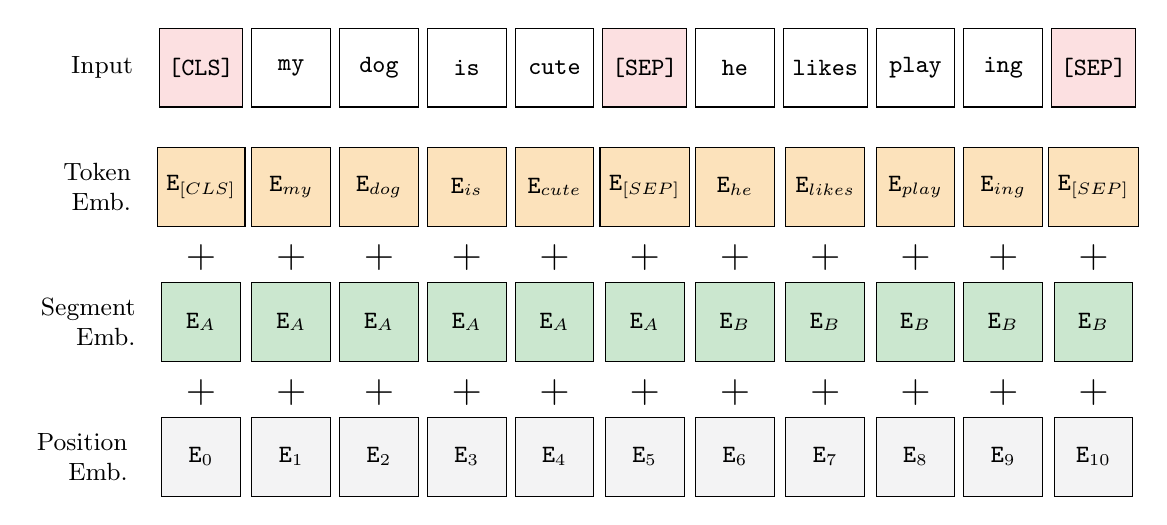
\begin{tikzpicture}[node distance=0.1cm, start chain=1 going right]

% Input boxes
\node [on chain=1, box, fill=customBlue] (in1) {[CLS]};
\node [on chain=1, box] (in2) {my};
\node [on chain=1, box] (in3) {dog};
\node [on chain=1, box] (in4) {is};
\node [on chain=1, box] (in5) {cute};
\node [on chain=1, box, fill=customBlue] (in6) {[SEP]};
\node [on chain=1, box] (in7) {he};
\node [on chain=1, box] (in8) {likes};
\node [on chain=1, box] (in9) {play};
\node [on chain=1, box] (in10) {ing};
\node [on chain=1, box, fill=customBlue] (in11) {[SEP]};

% Token Embeddings
\node [below=0.5cm of in1, emb] (E1) {E$_{[\text{CLS}]}$};
\node [below=0.5cm of in2, emb] (E2) {E$_{my}$};
\node [below=0.5cm of in3, emb] (E3) {E$_{dog}$};
\node [below=0.5cm of in4, emb] (E4) {E$_{is}$};
\node [below=0.5cm of in5, emb] (E5) {E$_{cute}$};
\node [below=0.5cm of in6, emb] (E6) {E$_{[\text{SEP}]}$};
\node [below=0.5cm of in7, emb] (E7) {E$_{he}$};
\node [below=0.5cm of in8, emb] (E8) {E$_{likes}$};
\node [below=0.5cm of in9, emb] (E9) {E$_{play}$};
\node [below=0.5cm of in10, emb] (E10) {E$_{ing}$};
\node [below=0.5cm of in11, emb] (E11) {E$_{[\text{SEP}]}$};

% Plus signs
\node [below=0.1cm of E1, plus] {+};
\node [below=0.1cm of E2, plus] {+};
\node [below=0.1cm of E3, plus] {+};
\node [below=0.1cm of E4, plus] {+};
\node [below=0.1cm of E5, plus] {+};
\node [below=0.1cm of E6, plus] {+};
\node [below=0.1cm of E7, plus] {+};
\node [below=0.1cm of E8, plus] {+};
\node [below=0.1cm of E9, plus] {+};
\node [below=0.1cm of E10, plus] {+};
\node [below=0.1cm of E11, plus] {+};

% Segment Embeddings
\node [below=0.7cm of E1, segA] (SA1) {E$_A$};
\node [below=0.7cm of E2, segA] (SA2) {E$_A$};
\node [below=0.7cm of E3, segA] (SA3) {E$_A$};
\node [below=0.7cm of E4, segA] (SA4) {E$_A$};
\node [below=0.7cm of E5, segA] (SA5) {E$_A$};
\node [below=0.7cm of E6, segA] (SA6) {E$_A$};
\node [below=0.7cm of E7, segB] (SB7) {E$_B$};
\node [below=0.7cm of E8, segB] (SB8) {E$_B$};
\node [below=0.7cm of E9, segB] (SB9) {E$_B$};
\node [below=0.7cm of E10, segB] (SB10) {E$_B$};
\node [below=0.7cm of E11, segB] (SB11) {E$_B$};

% Plus signs
\node [below=0.1cm of SA1, plus] {+};
\node [below=0.1cm of SA2, plus] {+};
\node [below=0.1cm of SA3, plus] {+};
\node [below=0.1cm of SA4, plus] {+};
\node [below=0.1cm of SA5, plus] {+};
\node [below=0.1cm of SA6, plus] {+};
\node [below=0.1cm of SB7, plus] {+};
\node [below=0.1cm of SB8, plus] {+};
\node [below=0.1cm of SB9, plus] {+};
\node [below=0.1cm of SB10, plus] {+};
\node [below=0.1cm of SB11, plus] {+};

% Position Embeddings
\node [below=0.7cm of SA1, posi] (P1) {E$_0$};
\node [below=0.7cm of SA2, posi] (P2) {E$_1$};
\node [below=0.7cm of SA3, posi] (P3) {E$_2$};
\node [below=0.7cm of SA4, posi] (P4) {E$_3$};
\node [below=0.7cm of SA5, posi] (P5) {E$_4$};
\node [below=0.7cm of SA6, posi] (P6) {E$_5$};
\node [below=0.7cm of SB7, posi] (P7) {E$_6$};
\node [below=0.7cm of SB8, posi] (P8) {E$_7$};
\node [below=0.7cm of SB9, posi] (P9) {E$_8$};
\node [below=0.7cm of SB10, posi] (P10) {E$_9$};
\node [below=0.7cm of SB11, posi] (P11) {E$_{10}$};

% Annotations
\node[left=0.2cm of in1, align=right, font=\small]{Input};
\node [left=0.2cm of E1, align=right, font=\small] {Token\\Emb.};
\node [left=0.2cm of SA1, align=right, font=\small] {Segment\\Emb.};
\node [left=0.3cm of P1, align=right, font=\small] {Position\\Emb.};

\end{tikzpicture}

    \caption[Input representation of BERT]{Input representation of BERT. The
    input is amended with special tokens \texttt{[CLS]} and \texttt{[SEP]} for
    NSP and represented as the sum of token, segment and positional embeddings.
    Figure adapted from \cite{devlin2019bert}.}
    \label{fig:bert_input}
\end{figure}

In the NSP task, BERT is presented with a pair of sentences and is tasked with
predicting whether the second sentence follows the first in the training corpus
or are a pair of unrelated sentences. In BERT, half of the training pairs were
positive pairs, while the other half had the second sentence randomly chosen
from different parts of the training corpus. To facilitate the NSP objective,
the token sequence preprocessing is slightly modified as shown in
Fig.~\ref{fig:bert_input}. BERT's input representation enriches the token
embeddings with the known positional embeddings (for reasons explained in
Sec.~\ref{subsec:input_emb}) but also adds segment embeddings. The latter
assists the model in the NSP task to distinguish between sentence membership of
tokens. Moreover, the input sequence is amended with two special tokens:
\texttt{[CLS]} indicating the beginning of the input sentence pair and
\texttt{[SEP]} separating the two sentences and marking the end of the input
pair. 

The final embedding of the \textbf{classification token}
$\bm{o}_{\texttt{[CLS]}}$ represents the next sentence prediction. In order to
compute a two-class prediction, a special \textbf{NSP head} is added to the
model, which consists of a linear layer with a learned set of classification
weights $\bm{W}_{NSP} \in \mathbb{R}^{d_{model} \times 2}$ followed by a softmax
activation function. The result is the binary prediction $\bm{\hat{y}}_i \in
\mathbb{R}^2$ for sentence pair $i$:

\begin{equation}
    \bm{\hat{y}}_i = \text{softmax}(\bm{o}_{\texttt{[CLS]}} \bm{W}_{NSP})
\end{equation}

As with the MLM task, cross-entropy is used to compute the NSP loss between the
actual \textit{one-hot encoded} label $\bm{y}_i$ and the predicted binary
probability distribution $\bm{\hat{y}}_i$. The total NSP loss is the sum of the
losses for all sentence pairs in the training set:

\begin{equation}
    \mathcal{L}_{NSP} = -\sum_{i} \bm{y}_i \log \bm{\hat{y}}_i, \quad \bm{y}_i \in \{[0, 1]^T, [1, 0]^T\}
\end{equation}

In pre-training, the final loss function for BERT is the sum of the MLM and NSP
losses, respectively:

\begin{equation}
    \mathcal{L}_{BERT} = \mathcal{L}_{MLM} + \mathcal{L}_{NSP}
\end{equation}

\begin{figure}[htb]
    \centering
    \includegraphics[width=0.5\textwidth]{figures/bert}
    \caption[Overview of the pre-training process of BERT]{Overview of the
    pre-training process of BERT, illustrating the MLM and NSP tasks. Input
    token sequences are amended with \texttt{[CLS]}, \texttt{[SEP]} and
    \texttt{[MASK]} tokens for masked token prediction and sentence pair
    coherence evaluation. Figure taken from \cite{devlin2019bert}.}
    \label{fig:bert}
\end{figure}

Fig.~\ref{fig:bert} summarizes BERT's pre-training process with all the
preprocessing steps and two learning objectives as described above. BERT was
pre-trained on the \textit{BookCorpus} \cite{zhu2015aligning} dataset and
English \textit{Wikipedia}, totaling to 16 GB of raw text, for approximately 40
epochs. Leveraging the large-scale pre-training data to extract rich contextual
word representations, BERT can be fine-tuned on numerous NLP tasks by adding
a lightweight task-specific output layer and training its parameters on the
target dataset, while freezing the pre-trained BERT weights. As a result,
fine-tuning is relatively inexpensive compared to pre-training. At the time of
its introduction, BERT surpassed all existing language models in various tasks,
establishing itself as the leading state-of-the-art NLP model.

\subsection{RoBERTa} \label{sec:roberta} 

RoBERTa (Robustly optimized BERT approach) forms the basis of this work's model
and is an optimized version of BERT introduced in the replication study
\cite{liu2019roberta}. RoBERTa and BERT share identical architecture and model
sizes, with each model featuring its own vocabulary and tokenization scheme.
Upon observing that BERT was significantly undertrained, the authors proposed
improvements to the choice of pre-training data, procedure and hyperparameters
as detailed in the following.

\paragraph{Byte-level BPE vocabulary} Adapting the tokenization scheme of GPT-2
\cite{radford2019gpt2}, RoBERTa utilizes a larger $|V| = 50,000$ byte-level BPE
(refer to Sec.~\ref{subsec:bbpe}). Compared to BERT's character-level WordPiece
vocabulary, this BPE vocabulary leverages the advantages of a subword
tokenization algorithm with the generality of a universal byte-level encoding
scheme, which is able to accommodate any Unicode character.

\paragraph{Pre-training data} As developing BERT-style LMs heavily relies on
large quantities of text, with direct impact on model performance, the authors
extended pre-training data size from 16 GB to 160 GB. The larger corpus consists
of five uncompressed English-language text corpora from multiple domains:

\begin{itemize}
    \item \textsc{BookCorpus}~\cite{zhu2015aligning}+\textsc{Wikipedia}, the
    identical datasets used for BERT (16 GB).
    \item \textsc{CC-News}, the authors created an own dataset based on the
    English portion of CommonCrawl~\cite{nagel2016common}, containing 63 million
    news articles (76 GB).
    \item \textsc{OpenWebText}~\cite{gokaslan2019OpenWeb}, a dataset compiled
    from Reddit outbound links with at least three up votes. An open source
    recreation of the WebText dataset used in GPT-2~\cite{radford2019gpt2} (38
    GB).
    \item \textsc{Stories}~\cite{trinh2018simple}, a collection of short
    narrative texts extracted from CommonCrawl~\cite{nagel2016common} (31 GB).
\end{itemize}

\paragraph{Dynamic masking for MLM} In the original BERT implementation, token
masking was performed once during data preprocessing for the MLM learning
objective, thus resulting in the same \textit{static} mask used across all
epochs. RoBERTa introduces a \textit{dynamic} masking strategy, where the mask
is randomly sampled for each training instance. The authors argue that this
modification improves the learning signal provided to the model by exposing it
to a more diverse set of training examples.

\paragraph{Removal of NSP task} The authors of RoBERTa found that the NSP task
did not provide any significant improvement in model performance on downstream
tasks. As a result, RoBERTa removes the NSP task from the pre-training process,
solely employing dynamic masked MLM as its training objective. At the same time,
preprocessing training data for RoBERTa, omits the inclusion of segment
embeddings and the usage of the \texttt{[CLS]} token for NSP prediction. Note,
that the training inputs for RoBERTa consist of full sentences extracted
consecutively from one or more documents, such that the total length does not
exceed the \textit{maximum input length} of 512 tokens. Whenever sentences in a
training example span over multiple documents, the \texttt{[SEP]} token is used
as a separator between text segments from different documents. This is done to
ensure consistent batch sizes when pre-training, which leads to improved model
training efficiency. For the remainder of this thesis, we refer to the described
procedure of packing text sequences from multiple documents as
\textbf{Full-Sentences}.

\paragraph{Larger batch sizes} The experiments compared the effect of batch size
on optimization speed and model performance. While the original BERT was trained
for one million steps with a batch size of 256 sequences, the authors compared
using the computationally equivalent combination of a batch size of 8,192
sequences and 31,000 training steps with tuned learning rate. The results showed
that larger batch sizes are beneficial in terms of perplexity when the learning
rate is adjusted appropriately. The final RoBERTa model adapted the larger batch
size of 8,192 sequences, while increasing the number of training steps to
500,000, concluding that the original BERT model was indeed undertrained.

Furthermore, larger batch sizes are more easily parallelizable across multiple
GPUs using data parallel training. Even without extensive parallel hardware,
larger batch sizes can enhance training efficiency by means of \textbf{gradient
accumulation} \cite{keskar2017large, ott2018scaling}. This technique simulates a
larger batch size by accumulating gradients computed for multiple mini-batches
locally before performing an optimization step. In practice, this allows for
performing an optimization step with a larger effective batch size, while
keeping the memory requirements of each mini-batch constant.
